\section{Preliminaries}\label{sec:prelims}
In this section we introduce the definitions and lemmas that we will use to
develop and analyze our results throughout the paper.

\subsection{Graphs and betweenness centrality}\label{sec:graphprelims}
Let $G=(V,E)$ be a graph, where $E\subseteq V\times V$, with $n=|V|$ vertices
and $m=|E|$ edges. The graph $G$ can be directed or undirected. We assume that
there are no self-loops from one vertex to itself and no multiple edges between
a pair of vertices. Each edge $e\in E$ has a non-negative weight
$\mathsf{w}(e)$. Given a pair of distinct vertices $(u,v)\in V\times V$,
$u\neq v$, a \emph{path $p_{uv}\subseteq V$ from $u$ to $v$} is an ordered sequence of
vertices $p_{uv}=(w_1,\dotsc,w_{|p_{uv}|})$ such that $w_1=u$, $w_{|p_{uv}|}=v$ and
for each $1\le i < |p_{uv}|$, $(w_i,w_{i+1})\in E$. The vertices $u$ and $v$ are
called the \emph{end points} of $p_{uv}$ and the vertices in
$\mathsf{Int}(p_{uv})=p_{uv}\setminus\{u,v\}$ are the \emph{internal vertices of
$p_{uv}$}. The \emph{weight}
$\mathsf{w}(p_{uv})$ of a path $p_{uv}=(u=w_1,w_2,\cdots,w_{p_{|uv|}}=v)$ from
$u$ to $v$ is the sum of the weights of the edges composing the path:
$\mathsf{w}(p_{uv})=\sum_{i=1}^{|p_{uv}|-1}\mathsf{w}((w_i,w_{i+1}))$. We denote with
$|p_{uv}|$ the number of vertices composing the path and call this the
\emph{size of the path $p_{uv}$}. Note that if the weights are not all unitary,
it is not necessarily true that $\mathsf{w}(p_{uv})=|p_{uv}|-1$. A special and
degenerate path is the \emph{empty path} $p_{\emptyset}=\emptyset$, which by
definition has weight $\mathsf{w}(p_\emptyset)=\infty$, no end points, and
$\mathsf{Int}(p_\emptyset)=\emptyset$.

Given two distinct vertices $(u,v)\in V\times V$, the \emph{shortest path distance}
$d_{uv}$ between $u$ and $v$ is the weight of a path with minimum weight 
between $u$ and $v$ among all paths between $u$ and $v$. If there is no path
between $u$ and $v$, $d_{uv}=\infty$. We call a path between $u$ and $v$ with
weight $d_{uv}$ a \emph{shortest path between $u$ and $v$}. There can be
multiple shortest paths between $u$ and $v$ and we denote the set of these paths
as $\mathcal{S}_{uv}$ and the number of these paths as
$\sigma_{uv}=|\mathcal{S}_{uv}|$. If there is no path between $u$ and $v$, then
$\mathcal{S}_{uv}=\{p_\emptyset\}$\footnote{Note that even if
$p_\emptyset=\emptyset$, the set $\{p_\emptyset\}$ is not empty. It contains
one element.}.
%By definition, $\mathcal{S}_{vv}=\emptyset$.
We denote with $\mathbb{S}_G$ the union of all the $\mathcal{S}_{uv}$'s, for all
pairs $(u,v)\in V\times V$ of distinct nodes $u\neq v$: 
\[ \mathbb{S}_G=\bigcup_{\substack{(u,v)\in V\times V \\ u\neq v}}\mathcal{S}_{uv}\enspace.\]

We now define a characteristic quantity of a graph that we will use throughout
the paper.
\begin{definition}\label{def:vertexdiam}
  Given a graph $G=(V,E)$, the \emph{vertex-diameter $\VD(G)$ of $G$} is the
  size of the shortest path in $G$ with maximum size:
  \[
  \VD(G) = \max\left\{|p| ~:~ p\in \mathbb{S}_G\right\}\enspace.\]
\end{definition}
The vertex-diameter is the maximum number of vertices among all shortest paths
in $G$. If all the edge weights are unitary, then $\VD(G)$ is equal to
$\mathsf{diam}(G)+1$, where $\mathsf{diam}(G)$ is the number of edges composing
the longest shortest path in $G$. 
%\XXX Shall we make an example with a figure?

Given a vertex $v$, let $\mathcal{T}_v\subseteq\mathbb{S}_G$ be the set of all
shortest paths that $v$ is \emph{internal} to:
\[
\mathcal{T}_v=\{p\in\mathbb{S}_G ~:~ v\in\mathsf{Int}(p)\}\enspace.
\]
In this work we are interested in the \emph{betweenness centrality} of the
vertices of a graph.

%\begin{definition}[\citep{Anthonisse71,Freeman77}]\label{def:betwenness}
\begin{definition}\label{def:betwenness}
  \citep{Anthonisse71,Freeman77} Given a graph $G=(V,E)$, the \emph{betweenness
  centrality of a vertex $v\in V$} is defined as\footnote{We use the normalized
  version of betweenness as we believe it to be more suitable for presenting
  approximation results.}
  \[
  \betw(v)=\frac{1}{n(n-1)}\sum_{p_{uw}\in\mathbb{S}_G}\frac{\mathds{1}_{\mathcal{T}_v}(p)}{\sigma_{uv}}%=\frac{1}{n(n-1)}\sum_{p_{uw}\in\mathcal{T}_v}\frac{1}{|\mathcal{S}_{uw}|}
  \enspace.
  \]
\end{definition} 

It is easy to see that $\betw(v)\in[0,1]$. \citet{Brandes01} presented an
algorithm to compute the betweenness centrality for all $v\in V$ in time
$O(nm)$ for unweighted graphs and $O(nm + n^2 \log n)$ for weighted graphs. 

\ifproof
\else
A ``local'' variant of betweenness, called \emph{$k$-bounded-distance
betweenness}\footnote{Bounded-distance betweenness is also known as
$k$-betweenness. We prefer the former denomination to avoid confusion with
$k$-path betweenness.} only considers
the contribution of shortest paths of size up to $k+1$~\citep{BorgattiE06,Brandes08}.
For $k>1$ and any pair of distinct vertices $u,v\in V$, $u\neq V$, let
$\mathcal{S}^{(k)}_{uv}\subseteq\mathcal{S}_{uv}$ be the set of shortest paths
from $u$ to $v$ of size at most $k+1$, with
$\sigma^{(k)}_{uv}=|\mathcal{S}^{(k)}_{uv}|$, and let $\mathbb{S}^{(k)}_G$ be the
union of all the $\mathcal{S}^{(k)}_{uv}$. Let
$\mathcal{T}^{(k)}_v\subseteq\mathcal{T}_v$ be the set of all shortest paths
\emph{of size up to $k$} that $v$ is internal to, for each $v\in V$.

%\begin{definition}[\citep{BorgattiE06,Brandes08}]\label{def:kboundbetweenness}
\begin{definition}\label{def:kboundbetweenness}
  \citep{BorgattiE06,Brandes08} Given a graph $G=(V,E)$ and an integer $k>1$,
  the \emph{$k$-bounded-distance betweenness centrality of a vertex $v\in V$} is
  defined as
  \[
  %\betw(v)=\sum_{(u,w)\in V\times
  %V}\sum_{p\in\mathcal{S}_{uw}}\frac{\mathds{1}_{\mathcal{T}_v}(p)}{|\mathcal{S}_{uw}|}\enspace.
  %\betw(v)=\sum_{p_{uw}\in\mathbb{S}_G}\frac{\mathds{1}_{\mathcal{T}_v}(p)}{|\mathcal{S}_{uw}|}\enspace.
  \kboundbetw^{(k)}(v)=\frac{1}{n(n-1)}\sum_{p_{uw}\in\mathbb{S}^{(k)}_G}\frac{\mathds{1}_{\mathcal{T}^{(k)}_v}(p)}{\sigma^{(k)}_{uw}}
  %=\frac{1}{n(n-1)}\sum_{p_{uw}\in\mathcal{T}^{(k)}_v}\frac{1}{\left|\mathcal{S}^{(k)}_{uw}\right|}
  \enspace.
  \]
\end{definition}
\fi

\subsection{Vapnik-Chervonenkis dimension}\label{sec:prelvcdim}
The Vapnik-Chernovenkis (VC) dimension of a class of subsets defined
on a set of points is a measure of the complexity or expressiveness of such
class~\citep{VapnikC71}. Given a probability distribution on the set of points,
a finite bound on the VC-dimension of the class of subsets implies a bound on
the number of random samples required to approximate the probability of each
subset in the class with its empirical average. We outline here some basic
definitions and results and refer the reader to the book by~\citet{MohriRT12}
for an in-depth presentation.
%works of~\citet[Sect.~14.4]{AlonS08} and
%\citet[Sect.~3]{BoucheronBL05} for an introduction of VC-dimension and a survey
%of recent developments. \XXX Cite book Foundations of ML instead.
%~\citet[Sect.~12.4]{DevroyeGL96},
%\citet[Sect.~3]{BoucheronBL05}, \citet[Sect.~14.4]{AlonS08}, and
%\citet{Vapnik99} for more details on VC-dimension.

Let $D$ be a domain and $\range$ be a collection of subsets from $D$. We call
$\range$ a \emph{range set on $D$}.
Given $B\subseteq D$, the \emph{projection of $\range$ on $B$} is the set 
$P_\range(B)=\{ B\cap A ~:~ A\in\range\}$. We say that the set $B$ is
\emph{shattered} by $\range$ if $P_\range(B)=2^B$.

\begin{definition}\label{def:vcdim}
  The \emph{Vapnik-Chervonenkis (VC) dimension of $\range$}, denoted as
  $\VC(\range)$, is the cardinality of the largest subset of $D$ that is
  shattered by $\range$.
\end{definition}

\ifproof
Note that a range space $(X,R)$ with an arbitrary large set of points $X$ and
an arbitrary large family of ranges $R$ can have a bounded VC-dimension. A simple
example is the family of intervals in $[0,1]$ (i.e. $X$ is all the points in
$[0,1]$ and $R$ all the intervals $[a,b]$, such that $0\leq a\leq b\leq 1$). Let
$A=\{x,y,z\}$ be the set of three points $0<x<y<z<1$. No interval in $R$ can
define the subset $\{x,z\}$ so the VC-dimension of this range space is less than
3~\citep[Lemma 10.3.1]{Matousek02}. Another example is shown in
Fig.~\ref{fig:rectangles}.
\begin{figure}[ht]
  \centering
  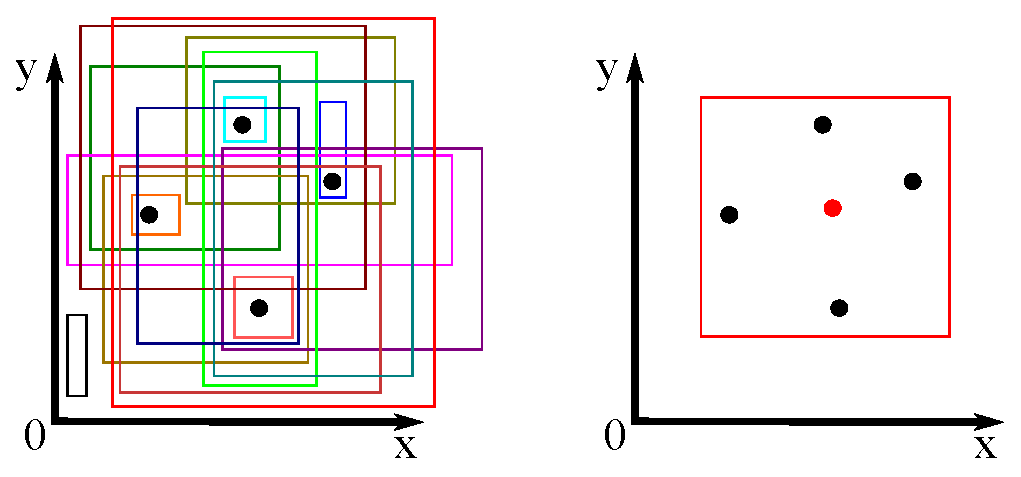
\includegraphics[width=.7\textwidth,keepaspectratio]{figures/rectangles}
  \caption{Example of range space and VC-dimension. The space of points is the
  plane $\mathbb{R}^2$ and the set of ranges is the set of all
  \emph{axis-aligned rectangles}. The figure on the left shows graphically that
  it is possible to shatter a set of four points using 16 rectangles. On the
  right instead, one can see that it is impossible to shatter five points, as,
  for any choice of the five points, there will always be one (the red point in
  the figure) that is internal to the convex hull of the other four, so it would
  be impossible to find an axis-aligned rectangle containing the four points
  but not the internal one. Hence $\VC((X,R))=4$.}
  \label{fig:rectangles}
\end{figure}
\fi

The main application of VC-dimension in statistics and learning
theory is in computing the number of samples needed to approximate the
probabilities of the ranges using their empirical averages as
unbiased estimators. Formally, let $X_1^k=(X_1,\dotsc,X_k)$ be a collection of
independent identically distributed random variables taking values in $D$,
sampled according to some distribution $\phi$ defined on the elements of $D$.
For a set $A\subseteq D$, let $\phi(A)$ be the probability that a sample from
$\phi$ belongs to the set $A$, and let the \emph{empirical average} of $\phi(A)$
on $X_1^k$ be 
\[
\phi_{X_1^k}(A)=\frac{1}{k}\sum_{j=1}^k\mathds{1}_A(X_j)\enspace.%, 
\]
%where $\mathds{1}_A$ is the indicator function for the set $A$. 
The empirical average of $\phi(A)$ can be used as an \emph{unbiased} estimator
for $\phi(A)$.

\begin{definition}\label{def:eapprox}
  Let $\range$ be a range set on %a domain
  $D$ and $\phi$ be a probability distribution on $D$. For $\varepsilon\in(0,1)$,
  an \emph{$\varepsilon$-approximation to $(\range,\phi)$} is a bag $S$ of
  elements of $D$ such that 
  \[
  \sup_{A\in\range}|\phi(A)-\phi_S(A)|\le\varepsilon\enspace.\]
\end{definition}

When an upper bound to the VC-dimension of $\range$ is available, it is possible
to build an $\varepsilon$-approximation by sampling points of
the domain according to the distribution $\phi$.

\begin{theorem}[Thm.~2.12~\citep{HarPS11} (see also~\citep{LiLS01})]\label{thm:eapprox}
  Let $\range$ be a range set on a domain $D$ with
  $\VC(\range)\le d$, and let $\phi$ be a distribution on $D$. Given
  $\varepsilon,\delta\in(0,1)$ let $S$ be a collection of $|S|$ points from $D$
  sampled according to $\phi$, with
  \begin{equation}\label{eq:vceapprox}
	|S|=\frac{c}{\varepsilon^2}\left(d+\ln\frac{1}{\delta}\right)
  \end{equation}
  where $c$ is an universal positive constant. Then $S$ is an
  $\varepsilon$-approximation to $(\range,\phi)$ with probability at least
  $1-\delta$.
\end{theorem}
%\XXX This is always a weird sentence that reviewers don't get. We should phrase it differently.
The constant $c$ is approximately $0.5$~\citep{LofflerP09}.
%\citet{LofflerP09} showed experimentally that the constant $c$ is approximately
%$0.5$. We used this value in our experiments.
%A similar definition offers relative guarantees on the approximation.
It is possible to obtain \emph{relative} guarantees on the approximation.
\begin{definition}\label{def:releapprox}
  Let $\range$ be a range set on $D$ and $\phi$ be a probability distribution on
  $D$. For $p,\varepsilon\in (0,1)$, a \emph{relative
  $(p,\varepsilon)$-approximation to $(\range,\phi)$} is a bag $S$ of elements
  from $D$ such that 
  \begin{itemize}
    \item For any $A\in\range$ such that $\phi(A)\ge p$, we have 
      \[ |\phi(A) - \phi_S(A)|\le \varepsilon\phi(A)\enspace.\]
    \item For any $B\in\range$ such that $\phi(B)< p$, we have $\phi_S(B)\le
      (1+\varepsilon)p$.
  \end{itemize}
\end{definition}

\begin{theorem}[Thm.~2.11~\citep{HarPS11}]\label{thm:releapprox}
  Let $\range$ be a range set on a domain $D$ with
  $\VC(\range)\le d$, and let $\phi$ be a distribution on $D$. Given
  $\varepsilon,\delta,p\in(0,1)$ let $S$ be a collection of $|S|$ points from $D$
  sampled according to $\phi$, with 
  \begin{equation}\label{eq:releapprox}
    |S|\ge\frac{c'}{\varepsilon^2p}\left(d\log\frac{1}{p}+\log\frac{1}{\delta}\right)
  \end{equation}
  where $c'$ is an absolute positive constant. Then $S$ is a relative
  $(p,\varepsilon)$-approximation to $(\range,\phi)$ with probability at least
  $1-\delta$.
\end{theorem}

It is important to mention that if $\VC(\range)$ and/or the upper bound $d$ do
not depend on $|D|$ or on $|\range|$ neither do the sample sizes presented in
Thm.~\ref{thm:eapprox} and~\ref{thm:releapprox}. This will make our algorithms
scale well as the size of the network increases.

